\documentclass[pdflatex,compress,mathserif]{beamer}

%\usetheme[dark,framenumber,totalframenumber]{ElektroITK}
\usetheme[darktitle,framenumber,totalframenumber]{ElektroITK}

\usepackage[utf8]{inputenc}
\usepackage[T1]{fontenc}
\usepackage{lmodern}
\usepackage[bahasai]{babel}
\usepackage{amsmath}
\usepackage{amsfonts}
\usepackage{amssymb}
\usepackage{graphicx}
\usepackage{multicol}
\usepackage{lipsum}
\usefonttheme[onlymath]{serif}

\newcommand*{\Scale}[2][4]{\scalebox{#1}{$#2$}}%

\setbeamertemplate{caption}[numbered]

\title{Pengolahan Sinyal Digital}
\subtitle{Realisasi Filter Digital}

\author{Mifta Nur Farid}

\begin{document}

\maketitle

\section{Pendahuluan}

\begin{frame}
	\frametitle{Sub-CPMK}
	Mahasiswa mampu merealisasikan filter-filter digital berdasarkan fungsi transfer maupun karakteristik filter lainnya.
\end{frame}

\begin{frame}
	\frametitle{Bahan Kajian}
	\begin{itemize}
		\item Direct Realization
		\item Direct Canonic Realization
		\item State-Space Realization
		\item Lattice Realization
		\item Cascade Realization
		\item Parallel Realization
	\end{itemize}
\end{frame}

\begin{frame}
	\frametitle{Pengantar}
	\begin{itemize}
		\item Hal-hal yang telah kita pelajari:
		\begin{enumerate}
			\item Dasar-dasar dalam menganalisis suatu sinyal
			\item Karakterisasi dan analisis sistem waktu diskrit
		\end{enumerate}
		\item Selanjutnya akan kita bahas desain sistem waktu-diskrit yang dapat digunakan di dalam DSP.
		\item Langkah-langkah dalam mendesain filter digital
		\begin{enumerate}
			\item Aproksimasi
			\item Realisasi
			\item Analisis kesalahan aritmatika
			\item Implementasi
		\end{enumerate}
	\end{itemize}
\end{frame}

\begin{frame}{Pengantar}
	\begin{itemize}
		\item \textbf{Aproksimasi:}  menghasilkan fungsi transfer yang memenuhi spesifikasi yang diinginkan.
		\item Metode-metode aproksimasi dapat dikategorikan menjadi:
		\begin{enumerate}
			\item \textbf{Direct:} permasalahan diselesaikan secara langsung dalam domain-$ z $.
			\item \textbf{Indirect:} fungsi transfer waktu kontinyu didapatkan terlebih dahulu kemudian dikonversi ke dalam fungsi transfer waktu diskrit.
		\end{enumerate}
	\end{itemize}
\end{frame}

\begin{frame}{Pengantar}
	\begin{itemize}
		
		\item Metode-metode aproksimasi dapat dikategorikan menjadi:
		\begin{enumerate}
			\item \textbf{Closed-form:} permasalahan diselesaikan melalui beberapa langkah desain yang sedikit dan menggunakan beberapa persamaan \textit{closed-form}.
			\item \textbf{Iterative:} solusi awal diasumsikan terlebih dahulu, kemudian dengan menerapkan metode optimisasi, secara bertahap didapatkan solusi yang sesuai dengan spesifikasi yang diinginkan.
		\end{enumerate}
		\item Metode aproksimasi yang dipilih berdasarkan:
		\begin{enumerate}
			\item yang sederhana
			\item yang handal
			\item yang menghasilkan disain yang tepat
			\item membutuhkan usaha komputasi yang minimal, dst.
		\end{enumerate}
	\end{itemize}
\end{frame}

\begin{frame}{Pengantar}
	\begin{itemize}
		\item \textbf{Realisasi} atau \textbf{sintesis}: proses menghasilkan jaringan atau struktur filter digital dari fungsi transfer atau karakteristik lain dari filter.
		\item Metode-metode realisasi dapat dikategorikan menjadi
		\begin{enumerate}
			\item \textbf{Direct:} realisasi didapatkan secara langsung dari fungsi transfer waktu-diskrit yang diberikan.
			\item \textbf{Indirect:} realisasi didapatkan secara tidak langsung dari purwarupa filter analog yang ekivalen.
		\end{enumerate}
		\item Pemilihan metode realisasi berdasarkan:
		\begin{enumerate}
			\item yang mudah diimplementasikan ke dalam bentuk rangkaian very-large-scale integrated (VLSI)
			\item yang membutuhkan sedikit unit delay, adder, dan multiplier
			\item yang tidak terlalu dipengaruhi oleh penggunaan aritmatika finite-precision dalam implementasinya, dst.
		\end{enumerate}
	\end{itemize}
\end{frame}

\begin{frame}{Pengantar}
	\begin{itemize}
		\item Ketidaksempurnaan desain disebabkan oleh ketidakakuratan pemodelan, toleransi komponen-komponen, efek-efek nonlinear yang tidak biasa dan tidak terduga, dst.
		\item Desain akan diterima selama ketidaksempurnaan tersebut tidak mengganggu spesifikasi yang diinginkan.
		\item Di dalam filter digital, ketidaksempurnaan biasanya disebabkan oleh ketidaktepatan secara numerik. Sehingga perlu untuk dipelajari.
	\end{itemize}
\end{frame}

\begin{frame}{Pengantar}
	\begin{itemize}
		\item Pada tahap aproksimasi, koefisien dari fungsi transfer ditentukan menjadi presisi tingkat tinggi.
		\item Namun dalam praktiknya, perangkat-perangkat keras yang digital memiliki kepresisian terbatas yang bergantung pada
		\begin{enumerate}
			\item panjangnya register yang digunakan untuk menyimpan suatu nilai
			\item jenis sistem angka yang digunakan (signed-magnitude, 2's comlement)
			\item jenis aritmatik yang digunakan (fixed-point, floating-point), dst.
		\end{enumerate}
		\item Akibatnya, koefisien filter harus dikuantisasi (rounded/ pembulatan atau truncated) sebelum disimpan di dalam register.
	\end{itemize}
\end{frame}

\begin{frame}{Pengantar}
	\begin{itemize}
		\item Saat koefisien fungsi transfer dikuantisasi, kesalahan akan muncul di dalam amplitudo dan fasa respons dari filter, yang umumnya disebut sebagai kesalahan kuantisasi (quantization errors)
		\item Kesalahan tersebut dapat menyebabkan filter digital melanggar spesifikasi yang diinginkan dan dalam kasus yang lebih parah lagi dapat menyebabkan ketidaksetabilan.
		\item Oleh sebab itu, proses desain tidak dapat dianggap selesai sampai efek \textbf{kesalahan aritmatika} pada kinerja filter diselidiki dan ditemukan cara untuk mengurangi masalah yang terkait dengan ketidaktepatan numerik.
	\end{itemize}
\end{frame}

\begin{frame}{Pengantar}
	\begin{itemize}
		\item \textbf{Implementasi} filter digital dapat diasumsikan menjadi dua bentuk
		\begin{enumerate}
			\item \textbf{software:} melibatkan simulasi struktur filter pada general-purpose digital computer, workstation, atau chip DSP
			\item \textbf{hardware:} melibatkan konversi struktur filter menjadi perangkat keras khusus.
		\end{enumerate}
		\item Penerapan non-realtime $ \rightarrow $ software.
		\item Penerapan realtime $ \rightarrow $ hardware.
	\end{itemize}
\end{frame}

\section{Realisasi}

\begin{frame}
	\frametitle{Realisasi}
	\begin{itemize}
		\item Direct realization/ realisasi langsung yang paling banyak digunakan adalah
		\begin{enumerate}
			\item Direct
			\item Direct canonic
			\item State-space
			\item Lattice
			\item Parallel
			\item Cascade
		\end{enumerate}
		\item Indirect realization: struktur filter analog yang direpresentasikan oleh wave characterization, akan ditransformasikan menjadi struktur filter digital.
	\end{itemize}
\end{frame}

\begin{frame}
	\frametitle{Direct Realization}
	\begin{itemize}
		\item Sebuah filter yang dikarakterisasi oleh fungsi transfer orde-$ N $
		\begin{equation}\label{8.1a}
			H(z) = \frac{N(z)}{D(z)} = \frac{\sum\limits_{i=0}^{N}a_i z^{-i}}{1 + \sum\limits_{i=0}^{N}b_i z^{-i}}
		\end{equation}
	\end{itemize}
\end{frame}

\begin{frame}{Direct Realization}
	\begin{itemize}
		\item Persamaan (\ref{8.1a}) dapat direpresentasikan sebagai
		\begin{equation}\label{8.1b}
			\frac{Y(z)}{X(z)} = H(z) = \frac{N(z)}{D(z)} = \frac{N(z)}{1 + D'(z)}
		\end{equation}
		yang mana
		\begin{equation}\label{8.2a}
			N(z) = \sum\limits_{i=0}^N a_i z^{-i}
		\end{equation}
		\begin{equation}\label{8.2b}
			D'(z) = \sum\limits_{i=0}^N a_i z^{-i}
		\end{equation}
	\end{itemize}
\end{frame}

\begin{frame}{Direct Realization}
	\begin{itemize}
		\item Persamaan (\ref{8.1b}) dapat direpresentasikan sebagai
		\begin{align*}
			Y(z) &= N(z)X(z) - D'(z)Y(z)
		\end{align*}
		atau
		\begin{align*}
			Y(z) = U_1(z)+U_2(z)
		\end{align*}
		yang mana
		\begin{equation}\label{8.3a}
			U_1(z) = N(z)X(z)
		\end{equation}
		\begin{equation}\label{8.3b}
			U_2(z) = -D'(z)Y(z)
		\end{equation}
	\end{itemize}
\end{frame}

\begin{frame}{Direct Realization}
	\begin{itemize}
		\item Oleh karena itu, realisasi dari $ H(z) $ dapat di-breakdown menjadi realisasi dari 2 fungsi transfer yang lebih sederhana, $ N(z) $ dan $ -D'(z) $, seperti yang ditunjukkan oleh Gambar \ref{fig:8.1}
		\begin{figure}
			\centering
			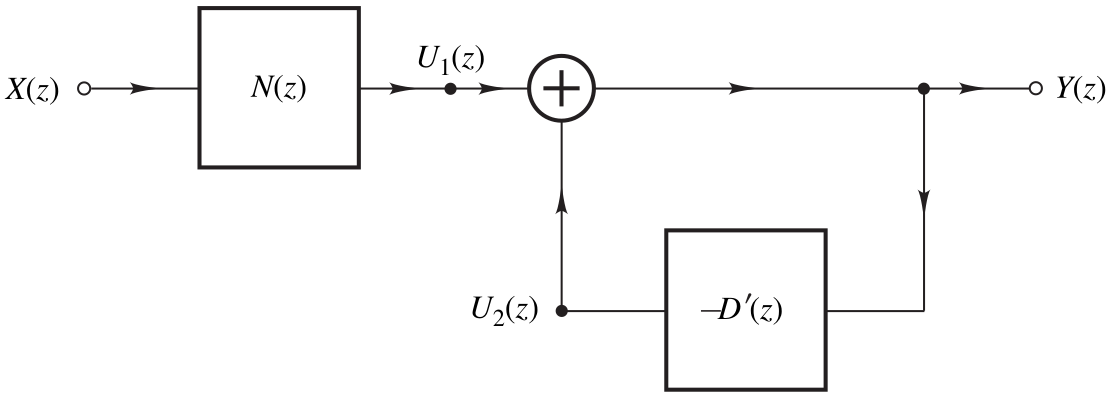
\includegraphics[width=\linewidth]{img/img01}
			\caption{Dekomposisi $ H(z) $ menjadi 2 fungsi transfer yang lebih sederhana}
			\label{fig:8.1}
		\end{figure}
		
	\end{itemize}
\end{frame}

\begin{frame}{Direct Realization}
	\begin{itemize}
		\item Misalkan realisasi dari $ N(z) $. Dari persamaan (\ref{8.2a}) dan (\ref{8.3a})
		\begin{align*}
			U_1(z) = \left[ a_0 + z^{-1} N_1(z) \right] X(z)
		\end{align*}
		yang mana
		\begin{align*}
			N_1(z) = \sum\limits_{i = 1}^{N}a_i z^{-i+1}
		\end{align*}
	\end{itemize}
\end{frame}

\end{document}
